\chapter{Related work}
\label{chap:rel_work}

\section{Linked Data}

This section presents a comprehensive exploration of Linked Data, encompassing its fundamental principles, data modeling, syntax, query interfaces, and the associated challenges and advantages. In Section~\ref{subsec:introduction_principles}, the concept of Linked Data and its principles are introduced, highlighting the significance of unique URIs, dereferencing, and data interlinking. Section~\ref{subsec:rdf} focuses on the Resource Description Framework (RDF) as the cornerstone for representing relationships and knowledge connections within Linked Data. Section~\ref{subsec:rdf_syntax} provides an overview of RDF syntax, including popular formats such as XML, Turtle, N-Triples, and JSON-LD, which facilitate the flexible expression and exchange of RDF data. Lastly, Section~\ref{subsec:sparql} briefly introduces SPARQL, the query language for RDF data This comprehensive examination serves as a solid foundation for the subsequent discussions on Linked Traversal-based Query Processing.

\subsection{Introduction and Principles}
\label{subsec:introduction_principles}

To better understand the origins of the idea behind Linked Data, it is important to examine the origins of the World Wide Web. For example, its first, but still rather primitive, underlying technology was introduced in 1989 at CERN. Tim Berners-Lee was the man responsible for its development. By using HyperText Markup Language (HTML), it enabled scientists, and later the rest of the world, to publish documents that could contain links to other documents. This helped create a mesh of documents and information. However, since these documents in fact contained nothing more than raw data dumps and links between documents represented simply an indication of how to reach the document, these documents and their relationships lacked semantics. Figure~\ref{fig:no_linked_data} illustrates what a web of documents without unambiguous indications of what their contents and the links between them represent, might look like. It is necessary to note here that the used icons are not the contents of their respective documents, but only a representation of their contents. Nevertheless, in themselves, they prove the weakness of such web as much as when the effective content of the documents had been represented. After all, just from the raw content of documents and their mutual links, a person cannot clearly infer exactly what their constellation represents, let alone a computer. From that deficiency, therefore, emerged the idea of Linked Data. \citep{jacksi2019development} \citep{bizer2011linked}

\begin{figure}[htbp]
    \centering
	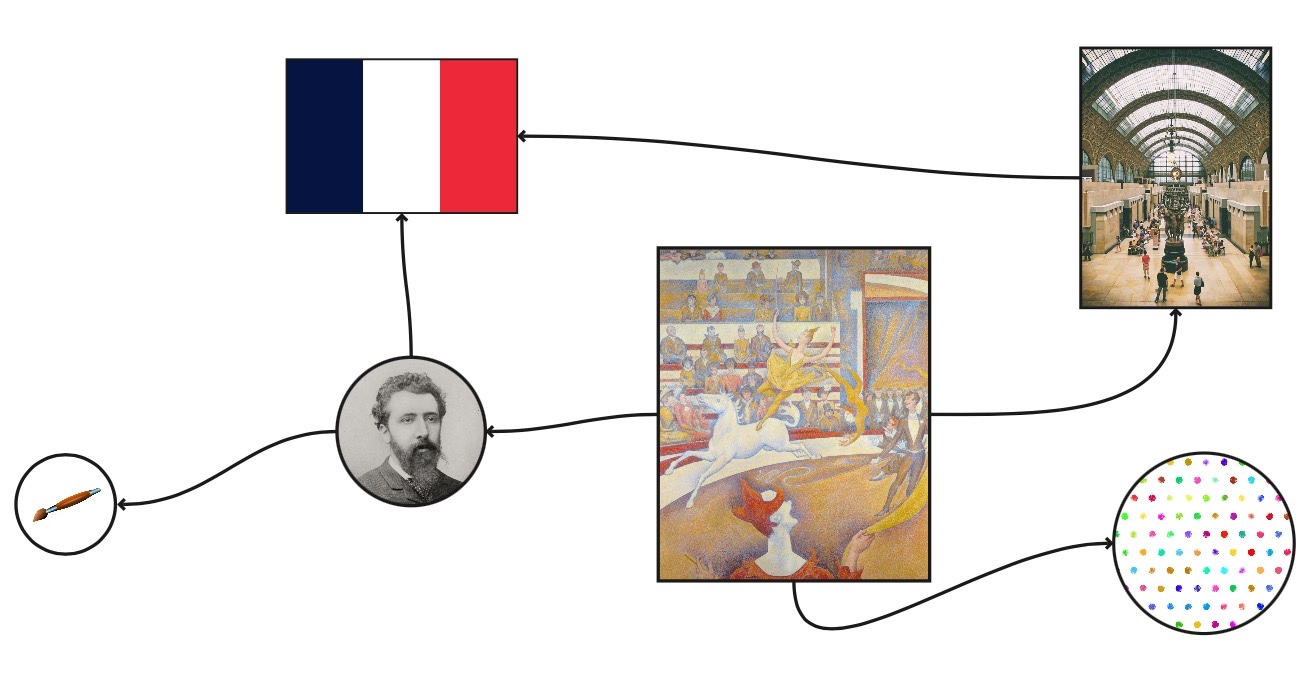
\includegraphics[width=\textwidth]{images/no_linked_data.jpg}
	\caption{Representation of a web of documents without unambiguous indications of what the documents and the links between them represent}
	\label{fig:no_linked_data}
\end{figure}

Simply put, data coming from different sources can be labeled as Linked Data as soon as they are linked by typed links. In other words, links are no longer just an indication of how to reach another document. Indeed, within the Linked Data story, they also contain information about what exactly the link in question represents. Linked Data thereby ensures the meaning of data is explicitly defined, in turn rendering the data machine-readable. Figure~\ref{fig:linked_data} represents the same web of documents as Figure~\ref{fig:no_linked_data}, but this time in accordance with the idea of Linked Data. Indeed, the documents have been given an  unambiguous indication of what they represent, and their mutual semantics have also been clarified thanks to the labeling of their links. \citep{bizer2011linked}

\begin{figure}[htbp]
    \centering
	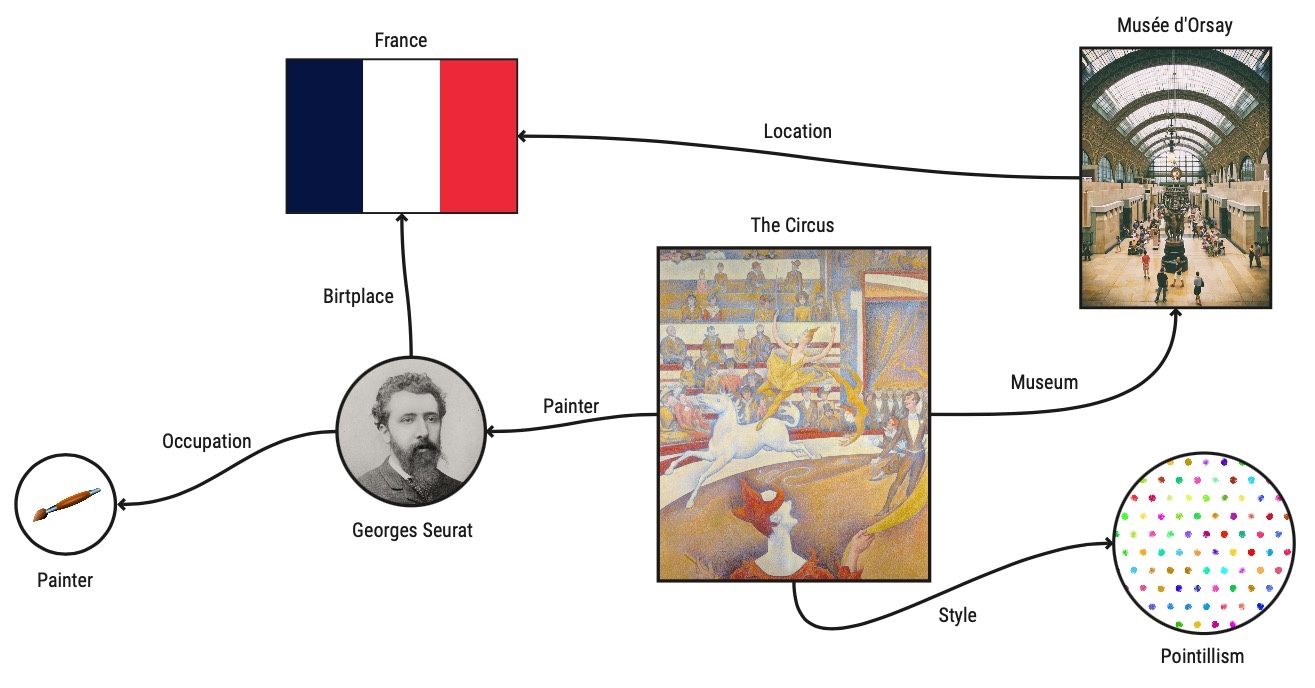
\includegraphics[width=\textwidth]{images/linked_data.jpg}
	\caption{Representation of a web of documents composed according to the spirit of Linked Data}
	\label{fig:linked_data}
\end{figure}

Although several technologies exist to achieve the goals of Linked Data, the use of URIs is essential. After all, since URIs are unique, they can unambiguously reference a particular entity. Practically speaking, the URIs that appear in a Linked Data document can be dereferenced using the HTTP protocol in order to retrieve the underlying entities. For instance, \mintinline{text}{https://stad.gent/id/concept/530010539}, is a URI that can be dereferenced using the HTTP(S) protocol. By dereferencing URI after URI in this way, little by little a - what could be called - \textit{field of information} unfolds, whose semantics can be unambiguously determined by both man and machine. \citep{bizer2011linked}

To clarify the concept of Linked Data, \citet{berners2006linked} put forth four principles to be taken into consideration.
\begin{enumerate}

    \item \textbf{Use URIs as names for things}\\
    The principle of using URIs has already been discussed above.
    
    \item \textbf{Use HTTP URIs so that people can look up those names}\\
    The principle of using the HTTP protocol to dereference URIs was also touched on above. Nevertheless, it is important to reiterate its importance, as there are other protocols besides HTTP for dereferencing URIs. However, these will technically differ from the HTTP protocol, each in its own different ways. For example, not using the ubiquitous Domain Name System (DNS), is, among others, a common practice among alternative protocols. However, in light of clarity and uniformity, as well as for other technical reasons, the HTTP protocol should be adhered to. \citep{berners2006linked}
    
    \item \textbf{When someone looks up a URI, provide useful information, using the standards (RDF, SPARQL)}\\
    Obviously, it would not fit within the spirit of Linked Data to obtain a raw data dump when dereferencing a URI that was included from another document as a \textit{Linked Data link}. The obtained data itself must comply with Linked Data principles. Therefore, there are some standards that clearly indicate how ontologies can be described. Consequently, to enable the construction of applications that deal with Linked Data, it goes without saying that a Linked Data document should be built according to the principles of an existing standard. RDF is the most common such standard and is therefore discussed further in Sections~\ref{subsec:rdf}. In addition, Section~\ref{subsec:sparql} introduces the SPARQL query interface. After all, large datasets are expected to also provide such interface. \citep{berners2006linked}
    
    \item \textbf{Include links to other URIs so that they can discover more things}\\
    The fourth and final principle, too, is rather obvious. After all, by definition, one can only speak of Linked Data when a document refers to at least one other document. In addition, to help advance the cause of transforming the World Wide Web in its current form into a semantic World Wide Web, aided by the concepts of Linked Data, it is preferable to also include links to documents belonging to other sites. \citep{berners2006linked}
    
\end{enumerate}

In conclusion, Linked Data plays a crucial role in giving meaning to the Web by enabling the interconnection and integration of diverse data sources. By adhering to the principles of unique URIs, dereferencing, linking, and using standardized formats, Linked Data fosters a more structured and interconnected web of knowledge. Examples such as DBpedia\footnote{\url{https://www.dbpedia.org}}, which provides a structured representation of Wikipedia data, and Friend of a Friend (FOAF), which allows for the description of people and their relationships, illustrate how publishing data as Linked Data benefits from enhanced data discoverability, interlinking with other datasets, and enabling novel applications and insights. Local initiatives like Collections of Ghent (CoGhent\footnote{\url{https://www.collections.gent}}), which digitizes art collections from cultural houses in Ghent and will be further discussed in Section~\ref{sec:coghent}, similarly demonstrate the potential of Linked Data for local organizations in contributing to the broader web of knowledge. \citep{auer2007dbpedia} \citep{golbeck2008linking} \citep{van2022publishing}

\subsection{Resource Description Framework}
\label{subsec:rdf}

The idea behind Linked Data is interesting in itself, but does not yet describe exactly how to get started with it. Therefore, this section introduces the Recourse Description Framework (RDF). Developed under the auspices of the World Wide Web Consortium (W3C), RDF is an infrastructure that allows for the construction of Linked Data datasets and their metadata. Consequently, this not only allows data publishers to lay out their data as Linked Data, but also gives data consumers clear guidance on how the data can be understood. Note here that data consumers can be both individuals and computer applications. \citep{miller1998introduction}

An interesting way to understand RDF is to first make a jump to the English language. Take the sentence below:
\begin{center}
    \textbf{The birthplace of Georges Seurat is France.}
\end{center}
According to English grammar, the \textit{who} or \textit{what} around which a sentence revolves, is called the subject of the sentence. Therefore, when looking at the sentence above, \textit{Georges Seurat} is its subject. In addition, the part of a sentence that gives more information about the subject, is referred to as the predicate, making \textit{the birthplace} the predicate in the above sentence. Finally, the matching value complementing the predicate and completing the sentence, is also of importance. Logically, in the case of the sentence above, that would be \textit{France}. Together, these three components form the most basic building blocks of a sentence. In fact, no matter their lengths, combined, they will always establish a piece of knowledge, exactly what RDF also seeks to accomplish. \citep{powers2003practical}

The building blocks of RDF data are basically exactly the same as those of linguistic sentences. After all, they are also three in number and even partly share the same names. Moreover, much like with sentences, combined, they form a single yet very clear piece of knowledge. Unlike the English language, however, they are not referred to as sentences. Rather, they are called triples. \citep{powers2003practical}
\begin{itemize}

    \item \textbf{Resource}\\
    \cite{miller1998introduction} defines a resource as any object that is uniquely identifiable by a URI. This enables it to come in different forms: as a web page, as an entire website or simply as any resource on the Web that conveys information in one way or another. \citep{candan2001resource}
    
    To make the comparison with the English language again, in a triple, the resource corresponds to the subject in a sentence. Moreover, in practice, the term \textit{subject} is often preferred over \textit{resource}. \citep{powers2003practical}

    \item \textbf{Property Type}\\
    A property type, or simply a property, introduces a specific aspect, characteristic, attribute, or relationship of a resource. A property type always expects a value to ultimately define the piece of knowledge represented by a triple. \citep{candan2001resource} \citep{miller1998introduction}
    
    As for property types, in practice, the corresponding term from the English language, \textit{predicate}, is also frequently used as opposed to the more theoretical \textit{property type}. \citep{powers2003practical}

    \item \textbf{Value}\\
    A value resolves the concept or relationship initiated by a property type. In this way, it captures the knowledge conveyed by the triple. Values can be represented as text strings, numbers, or any atomic data. However, they can also be resources themselves. This characteristic allows triples therefore to be the building blocks of a web of knowledge. \citep{miller1998introduction}
    
    It is evident that a value in a triple corresponds to a value in an English sentence. However, in practice, the term \textit{object} is often preferred. \citep{powers2003practical}
    
\end{itemize}

While triples convey a clear and distinct piece of knowledge, a collection of triples can naturally convey a more comprehensive knowledge. Such a collection of triples, interconnected by values that are themselves resources, is also referred to as an \textit{RDF description}. Figure~\ref{fig:rdf_description} illustrates what such an RDF description might look like. Additionally, it is important to note that each of its components, whether it be a resource, property type, or value, does not necessarily have to be a digital concept. After all, Web assets can perfectly represent real-life concepts. \citep{miller1998introduction} \citep{candan2001resource}

\begin{figure}[htbp]
    \centering
	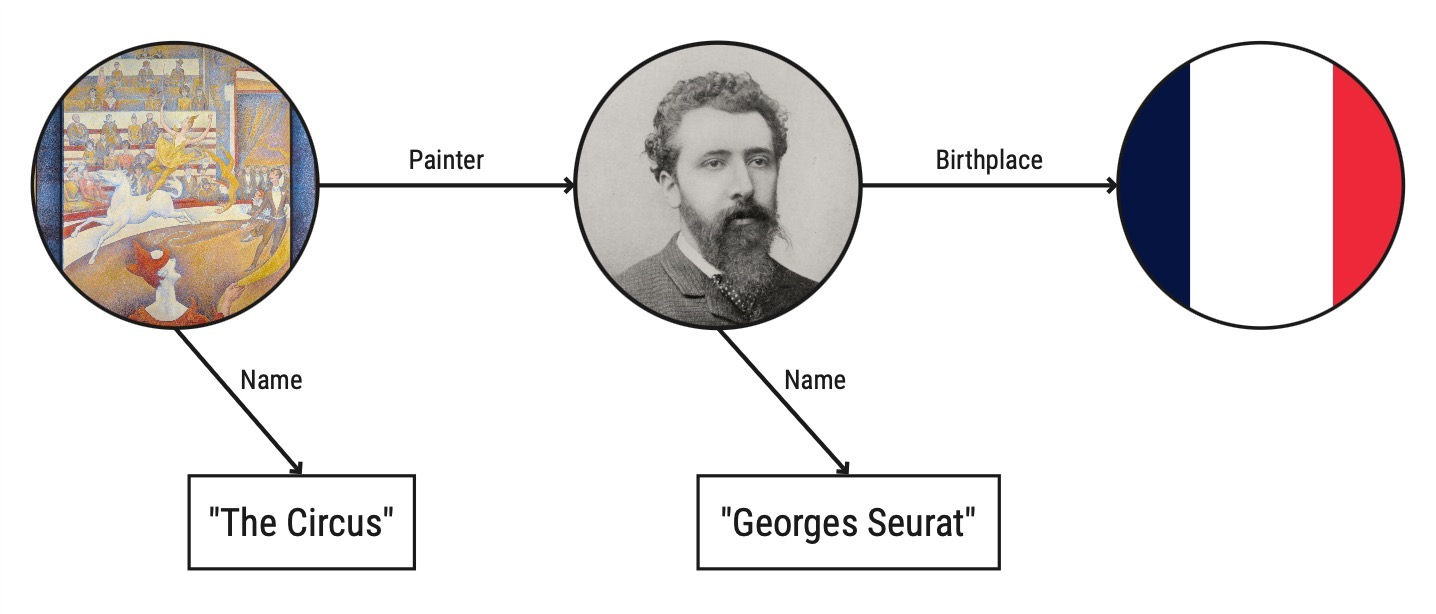
\includegraphics[width=\textwidth]{images/rdf_description.jpg}
	\caption{Representation of an RDF description}
    \caption*{Circles represent resources, arrows represent property types and values are situated at the end of arrows}
	\label{fig:rdf_description}
\end{figure}

Clearly, different terms exist to denote the same RDF concepts. For instance, in addition to the synonyms mentioned above, in literature, the term \textit{statement} is sometimes preferred over \textit{triple}. However, in light of uniformity and clarity, throughout the rest of this text, the terms \textit{triple}, \textit{subject}, \textit{predicate} and \textit{object} will be used instead of their counterparts. \citep{candan2001resource}

\subsection{Resource Description Framework Syntax}
\label{subsec:rdf_syntax}

What constitutes RDF exactly, should be clear by now, but the question of how to actually write down RDF descriptions, still remains to be answered. Therefore, this section introduces some RDF syntaxes. However, since they are not the focus of this research, they will not be discussed in detail. Instead, their outlines will be illustrated by presenting the RDF description from Figure~\ref{fig:rdf_description} in the syntax in question. Incidentally, since the schema presented in Figure~\ref{fig:rdf_description} also has clear guidelines on how to be used, in itself, it also qualifies as an RDF syntax, albeit a graphical one. \citep{miller1998introduction}

All the syntaxes to be discussed are instantiations of the RDF Model and Syntax Specification, providing concrete implementations. However, the first syntax stands apart from the rest as it primarily serves as a notation recommendation for humans to express RDF descriptions in a manner that is unambiguous yet simple. Unlike the other syntaxes, this particular one is not intended for machine consumption. Code Fragment~\ref{lst:human_rdf_syntax} demonstrates how the RDF description, as schematically depicted in Figure~\ref{fig:rdf_description}, can be represented using this human-centric syntax. In this representation, resources are enclosed in straight brackets, while property types are represented by arrows. Furthermore, the representation of values varies depending on their types. As denoted, resources are encapsulated within brackets. However, if the values are atomic in nature, they are simply enclosed in quotation marks. \citep{miller1998introduction}

\begin{listing}[htbp]
    \begin{minted}[samepage,fontsize=\small]{text}
[The Circus] ------name--------> "The Circus"
[The Circus] ------painter-----> [Georges Seurat]
[Georges Seurat] --name--------> "Georges Seurat"
[Georges Seurat] --birthplace--> [France]
    \end{minted}
    \caption{RDF description depicted using a human-centric RDF syntax}
    \label{lst:human_rdf_syntax}
\end{listing}

The example from Code Fragment~\ref{lst:human_rdf_syntax} is easy to read, but at the same time rather confusing. Indeed, certain resource names correspond to certain atomic values. One could of course try to give the resources a more generic name to indicate what exactly the resource in question means. However, that would make little sense given the way the following machine-readable RDF syntaxes refer to resources. After all, they use URIs, allowing for a more clear distinction between resources and atomic values.

\begin{itemize}

    \item \textbf{N-Triples}\\
    Code Fragment~\ref{lst:n_triples_syntax} depicts the representation of the RDF description using N-Triples. In this syntax, each line corresponds to a triple, wherein the subject, predicate, and object are delimited by spaces or tabs. The triple is terminated by a period and a new line character. \citep{seaborne2014rdf}

    \begin{listing}[htbp]
        \begin{minted}[samepage,fontsize=\footnotesize]{turtle}
<http://example.org/The_Circus> <http://example.org/name> "The Circus" .
<http://example.org/The_Circus> <http://example.org/painter> <http://example.org/Georges_Seurat> .
<http://example.org/Georges_Seurat> <http://example.org/name> "Georges Seurat" .
<http://example.org/Georges_Seurat> <http://example.org/birthplace> <http://dbpedia.org/resource/France> .
        \end{minted}
        \caption{RDF description depicted using the N-Triples syntax}
        \label{lst:n_triples_syntax}
    \end{listing}
    
    Furthermore, absolute URIs are employed to denote resources, while atomic values are enclosed within quotation marks. With that in mind, it is important to note that if a value itself contains a quotation mark, it must be properly escaped to ensure correct interpretation. \citep{seaborne2014rdf}

    \item \textbf{N3}\\
    Parsing an RDF description in N-Triples syntax is relatively straightforward for computers, but it can be challenging for humans to comprehend at a glance. The use of absolute URIs in N-Triples can lead to visual clutter and hinder readability. To address this, the N3 syntax builds upon N-Triples by introducing the concept of relative URIs. \citep{seaborne2014rdf}

    In N3, it is possible to specify a base URI by including a \mintinline{text}{@base <URI>} directive at the beginning of the document. When a relative URI is encountered elsewhere in the document, the parser appends it to the specified base URI. This allows for a more concise representation of URIs. \citep{berners2011notation3}

    However, RDF descriptions may contain URIs with different base URIs, making a single base URI insufficient. To overcome this limitation, N3 allows the document to be preceded by one or more \mintinline{text}{@prefix prefix: <URI>} directives. These directives associate prefixes with URIs, and the parser appends any relative URI preceded by a prefix to the corresponding base URI associated with that prefix. This mechanism enables the use of multiple base URIs within the same document and enhances the flexibility and expressiveness of the N3 syntax. Code Fragment~\ref{lst:n3_turtle_syntax} illustrates the use of prefixes for the N3 syntax.  \citep{berners2011notation3}

    \begin{listing}[htbp]
        \begin{minted}[samepage,fontsize=\small]{turtle}
@prefix ex: <http://example.org/> .
@prefix dbp: <http://dbpedia.org/resource/> .

ex:The_Circus ex:name "The Circus" .
ex:The_Circus ex:painter ex:Georges_Seurat .
ex:Georges_Seurat ex:name "Georges Seurat" .
ex:Georges_Seurat ex:birthplace dbp:France .
        \end{minted}
        \caption{RDF description depicted using the N3 and Turtle syntaxes}
        \label{lst:n3_turtle_syntax}
    \end{listing}

    \item \textbf{Turtle}\\
    The Turtle syntax is very similar to N3. In fact, Turtle is a subset of N3. Specifically, Code Fragment~\ref{lst:n3_turtle_syntax} can be processed by a Turtle parser just as well. However, while N3 allows for more expressiveness in principle, Turtle keeps things simpler, making it a popular choice for human readability. \citep{berners2011notation3} \citep{prudhommeaux2014turtle}

    Providing an exhaustive list of the precise differences between the two syntaxes would exceed the scope of this text since the intricacies of RDF syntaxes are not the primary focus here.

    \item  \textbf{RDF/XML}\\
    RDF/XML is one of the earliest RDF syntaxes and remains widely used. To introduce this syntax, Code Fragment~\ref{lst:xml_syntax} serves as a guide.

    \begin{listing}[htbp]
        \begin{minted}[samepage,fontsize=\small]{xml}
<rdf:RDF xmlns:rdf="http://www.w3.org/1999/02/22-rdf-syntax-ns#"
         xmlns:ex="http://example.org/"
         xmlns:dbp="http://dbpedia.org/resource/">
  <rdf:Description rdf:about="http://example.org/The_Circus">
    <ex:name>The Circus</ex:name>
    <ex:painter rdf:resource="http://example.org/Georges_Seurat"/>
  </rdf:Description>
  <rdf:Description rdf:about="http://example.org/Georges_Seurat">
    <ex:name>Georges Seurat</ex:name>
    <ex:birthplace rdf:resource="http://dbpedia.org/resource/France"/>
  </rdf:Description>
</rdf:RDF>
        \end{minted}
        \caption{RDF description depicted using the RDF/XML syntax}
        \label{lst:xml_syntax}
    \end{listing}

    The RDF description in RDF/XML is enclosed within \mintinline{text}{rdf:RDF} elements, where necessary prefixes can also be defined. While an XML declaration like \mintinline{text}{<?xml version="1.0"?>} can precede the RDF/XML document, it is optional and omitted in Code Fragment~\ref{lst:xml_syntax} to focus primarily on the basics of RDF syntaxes. \citep{gandon2014xml}

    Upon encountering the \mintinline{text}{rdf:RDF} tag, a parser recognizes that it should process an RDF description. In RDF/XML, such an RDF description is constructed using one or more \mintinline{text}{rdf:Description} elements. In fact, each \mintinline{text}{rdf:Description} element represents a subject, and its optional \mintinline{text}{rdf:about} attribute denotes the subject's URI. Consequently, the triples associated with the subject are enclosed within the corresponding \mintinline{text}{rdf:Description} tags. Predicates on the one hand, whether represented using a prefix or not, have their own elements. The representation of subjects, on the other hand, depends on their nature: for atomic values, they can simply be placed between opening and closing subject tags, while for resource subjects, their URIs are included as the value of an \mintinline{text}{rdf:resource} attribute within the subject tag. \citep{gandon2014xml}

    Once again, it is important to note that the Code Fragments used in this section provide only an introductory glimpse of the proposed syntaxes. They cover only a small portion of the potential scope of a syntax. Code Fragment~\ref{lst:xml_syntax}, in particular, demonstrates that RDF/XML syntax can obscure simplicity, especially when dealing with more extensive RDF descriptions. Consequently, RDF/XML is not commonly used for human-readable purposes but rather as a syntax primarily intended for machine consumption. \citep{dongo2019srdf}

    \item \textbf{JSON-LD}\\
    The final RDF syntax introduced is called JSON-LD. Similar to RDF/XML, JSON-LD builds upon an existing syntax for representing data on the web. However, JSON-LD representations are generally more human-readable. As most resources and examples in the following text will be presented in JSON-LD, a slightly more comprehensive overview of this syntax is provided compared to the previous ones. Nevertheless, what follows is not an exhaustive listing of all the intricacies of the syntax. Instead, it aims to offer readers a concise introduction to JSON-LD without prior knowledge, making the rest of the text more easily comprehensible. For those seeking more in-depth information about JSON-LD, it is recommended to consult other sources\footnote{The W3C JSON-LD 1.1 Recommendation provides very in-depth information about the JSON-LD syntax: \url{https://www.w3.org/TR/json-ld11/}.}.

    It is evident that the same data can be represented in various ways, and this applies to RDF data as well. While the visual representation of an RDF description, as depicted in Figure~\ref{fig:rdf_description}, is relatively straightforward, converting it into a fully textual format poses certain choices to be made. After all, there are numerous possibilities regarding the exact data representation. In the introduction of previous syntaxes, a specific representation was chosen each time. However, in this section, three different approaches for representing the same set of data using the JSON-LD syntax are presented.

    To start off, Code Fragment~\ref{lst:json_ld_nested_syntax} closely resembles the previous examples, using nesting to store all the data in a single JSON-LD document. However, some may question whether it is appropriate to make the \mintinline{text}{George_Seurat} resource a child of \mintinline{text}{The_Circus} resource, implying a hierarchical relationship that may not be relevant.

    \begin{listing}[htbp]
        \begin{minted}[samepage,fontsize=\small]{jsonld}
{
  "@context": {
    "ex": "http://example.org/",
    "dbp": "http://dbpedia.org/resource/"
  },
  "@id": "ex:The_Circus",
  "ex:name": "The Circus",
  "ex:painter": {
    "@id": "ex:Georges_Seurat",
    "ex:name": "Georges Seurat",
    "ex:birthplace": "dbp:France"
  }
}
        \end{minted}
        \caption{RDF description with nested objects depicted using the JSON-LD syntax}
        \label{lst:json_ld_nested_syntax}
    \end{listing}

    Subsequently, in Code Fragment~\ref{lst:json_ld_spread_syntax}, the data is split into two JSON-LD documents. Utilizing URIs, the documents can still refer to each other uniquely, without suggesting any hierarchical relationship between the resources.

    \begin{listing}[htbp]
        \begin{minted}[samepage,fontsize=\small,escapeinside=||]{jsonld}
|Document 1:|
{
  "@context": {
    "ex": "http://example.org/"
  },
  "@id": "ex:The_Circus",
  "ex:name": "The Circus",
  "ex:painter": "ex:Georges_Seurat"
}

|Document 2:|
{
  "@context": {
    "ex": "http://example.org/",
    "dbp": "http://dbpedia.org/resource/"
  },
  "@id": "ex:Georges_Seurat",
  "ex:name": "Georges Seurat",
  "ex:birthplace": "dbp:France"
}
        \end{minted}
        \caption{RDF description spread over two documents depicted using the JSON-LD syntax}
        \label{lst:json_ld_spread_syntax}
    \end{listing}

    Finally, Code Fragment~\ref{lst:json_ld_graph_syntax} takes a distinct approach by using the \mintinline{text}{@graph} property. This allows listing the necessary resources in a JSON array, placing them on equal footing within a single document. However, this method introduces extra clutter and overhead compared to the previous approaches. \citep{kellogg2020jsonld}

    Ultimately, the choice of representation depends on the specific use case and the desired balance between simplicity and expressiveness. Each approach has its advantages and trade-offs, showcasing the flexibility of the JSON-LD syntax in accommodating different data representation needs.

    \begin{listing}[htbp]
        \begin{minted}[samepage,fontsize=\small]{jsonld}
{
  "@context": {
    "ex": "http://example.org/",
    "dbp": "http://dbpedia.org/resource/"
  },
  "@graph": [
    {
      "@id": "ex:The_Circus",
      "ex:name": "The Circus",
      "ex:painter": {
        "@id": "ex:Georges_Seurat"
      }
    },
    {
      "@id": "ex:Georges_Seurat",
      "ex:name": "Georges Seurat",
      "ex:birthplace": {
        "@id": "dbp:France"
      }
    }
  ]
}
        \end{minted}
        \caption{RDF description as a graph depicted using the JSON-LD syntax}
        \label{lst:json_ld_graph_syntax}
    \end{listing}

    Understanding Code Fragments~\ref{lst:json_ld_nested_syntax}, \ref{lst:json_ld_spread_syntax}, and \ref{lst:json_ld_graph_syntax} becomes relatively straightforward after having discussed the previous syntaxes. However, two aspects deserve further attention: the use of \mintinline{text}{@id} and \mintinline{text}{@context} keywords in JSON-LD.

    Firstly, the \mintinline{text}{@id} keywords uniquely identify the proposed resources using URIs. Indeed, in the given examples, the id's do exactly that. \citep{kellogg2020jsonld}

    Secondly, the \mintinline{text}{@context} keyword plays a crucial role in JSON-LD. It introduces specifics that can be taken for granted in the actual data, reducing the need for repetitive information and cleaning up the actual JSON. While Code Fragments~\ref{lst:json_ld_nested_syntax}, \ref{lst:json_ld_spread_syntax}, and \ref{lst:json_ld_graph_syntax} use the context in a straightforward way by introducing prefixes, in practice, it can do more than that. Essentially, the context maps terms to URIs. These terms can be freely chosen to enhance human readability. \citep{kellogg2020jsonld}

    W3C's JSON-LD Recommendation\footnote{\url{https://www.w3.org/TR/json-ld11/}} offers a valuable example of how the context is typically used, as illustrated in Code Fragment~\ref{lst:json_ld_context}. The provided context clearly indicates that when the key \mintinline{text}{name} appears in the data, it refers to \mintinline{text}{http://schema.org/name}. Similarly, for \mintinline{text}{image} and \mintinline{text}{homepage}, their respective values are \textit{expanded} into objects that hold additional information. The \mintinline{text}{@type} keyword is also used in the example to indicate the type of the final value. In Code Fragment~\ref{lst:json_ld_context}, it shows that the \mintinline{text}{image} and \mintinline{text}{homepage} keys are followed by an \mintinline{text}{@id}, representing unique resources. Moreover, JSON-LD supports various other types, and custom types can be defined to suit specific requirements. \citep{kellogg2020jsonld}

    \begin{listing}[htbp]
        \begin{minted}[samepage,fontsize=\small]{jsonld}
{
  "@context": {
    "name": "http://schema.org/name",
    "image": {
      "@id": "http://schema.org/image",
      "@type": "@id"
    },
    "homepage": {
      "@id": "http://schema.org/url",
      "@type": "@id"
    }
  },
  "name": "Manu Sporny",
  "homepage": "http://manu.sporny.org/",
  "image": "http://manu.sporny.org/images/manu.png"
}
        \end{minted}
        \caption{Example of context use in JSON-LD, proposed by \cite{kellogg2020jsonld}}
        \label{lst:json_ld_context}
    \end{listing}

    To further enhance the cleanliness of a JSON-LD document, one can opt to store the context as a separate resource rather than embedding it directly in the document. Using this approach, the JSON-LD document includes the URI that references the context as the value for the \mintinline{text}{@context} key. Storing the context separately allows for greater modularity and reusability, making it easier to manage and maintain complex JSON-LD documents. The use of separate contexts can significantly improve the organization and readability of JSON-LD data, enhancing its compatibility with RDF and Linked Data principles. \citep{kellogg2020jsonld}

    To finish off this section on JSON-LD, it is interesting to note that when the JSON-LD document presented in Code Fragment~\ref{lst:json_ld_context} is \textit{expanded}, the data takes on its typical RDF form, adhering fully to the Linked Data principles. This expansion, as shown in Code Fragment~\ref{lst:json_ld_expanded}, reveals the underlying structure of the data and its connection to other resources. \citep{kellogg2020jsonld}

    \begin{listing}[htbp]
        \begin{minted}[samepage,fontsize=\small]{jsonld}
[{
  "http://schema.org/name": [{"@value": "Manu Sporny"}],
  "http://schema.org/url": [{ "@id": "http://manu.sporny.org/" }],
  "http://schema.org/image": [{ "@id": "http://manu.sporny.org/images/manu.png" }]
}]
        \end{minted}
        \caption{Example of an expanded JSON-LD document, proposed by \cite{kellogg2020jsonld}}
        \label{lst:json_ld_expanded}
    \end{listing}

    In summary, the \mintinline{text}{@id} and \mintinline{text}{@context} keywords in JSON-LD contribute to the readability, expressiveness, and flexibility of representing RDF data, enabling a more human-friendly approach to data serialization.
    
\end{itemize}

Before concluding this section on RDF syntaxes, it is crucial to reiterate that the explanations provided are not exhaustive. Only a surface-level overview of these syntaxes was covered, and there is much more to explore and learn about them. This section serves as a reference for those with limited or no prior knowledge of RDF syntaxes, aiming to facilitate their understanding of the remaining text. In the following sections, several RDF examples will be presented, with the majority of them using the JSON-LD syntax. However, there will be no further elaboration on new elements that are specific to each syntax unless they are essential for a clear understanding of the text. For readers seeking a more in-depth understanding of the syntaxes, additional resources are recommended to further explore their intricacies and capabilities.

\subsection{SPARQL}
\label{subsec:sparql}

TODO

\section{Link-Traversal-based Query Processing}
\label{sec:ltqp}

TODO

\section{Comunica}
\label{sec:comunica}

TODO

\section{Collections of Ghent}
\label{sec:coghent}

TODO

\subsection{Linked Data Event Streams}
\label{subsec:ldes}

\subsection{Example Queries}
\label{sec:coghent_example_queries}

TODO

\begin{listing}[htbp]
    \begin{minted}[fontsize=\small]{sparql}
PREFIX cidoc:<http://www.cidoc-crm.org/cidoc-crm/>
PREFIX adms:<http://www.w3.org/ns/adms#>
PREFIX skos:<http://www.w3.org/2004/02/skos/core#>
PREFIX la:<https://linked.art/ns/terms/>
SELECT ?title ?note ?image ?objectname ?objectnumber ?associatie
       ?creator ?plaats ?timespan ?techniek ?materiaal
WHERE {
    # Title
    ?o cidoc:P102_has_title ?title.
    # Description
    ?o cidoc:P3_has_note ?note.
    # Image
    ?o cidoc:P129i_is_subject_of ?image.
    # Objectname
    ?o cidoc:P41i_was_classified_by ?classified.
    ?classified cidoc:P42_assigned ?assigned.
    ?assigned skos:prefLabel ?objectname.
    # Association
    ?o cidoc:P128_carries ?carries.
    ?carries cidoc:P129_is_about ?about.
    ?about cidoc:P2_has_type ?type.
    ?type skos:prefLabel ?associatie.
    # Objectnumber
    ?o adms:identifier ?identifier.
    ?identifier skos:notation ?objectnumber.
    # Creator
    ?o cidoc:P108i_was_produced_by ?production.
    ?production cidoc:P14_carried_out_by ?producer.
    ?producer la:equivalent ?equivalent.
    ?equivalent rdfs:label ?creator.
    # Place
    ?o cidoc:P108i_was_produced_by ?produced.
    ?produced cidoc:P7_took_place_at ?tookplace.
    ?tookplace la:equivalent ?plaatsequivalent.
    ?plaatsequivalent skos:prefLabel ?plaats.
    # Date
    ?o cidoc:P108i_was_produced_by ?produced.
    ?produced cidoc:P4_has_time-span ?timespan.
    # Technique
    ?o cidoc:P108i_was_produced_by ?produced.
    ?produced cidoc:P32_used_general_technique ?technique.
    ?technique cidoc:P2_has_type ?hastype.
    ?hastype skos:prefLabel ?techniek.
    # Material
    ?o cidoc:P45_consists_of ?consists.
    ?consists cidoc:P2_has_type ?materiaaltype.
    ?materiaaltype skos:prefLabel ?materiaal.
}
    \end{minted}
    \caption{Example of SPARQL query created by original CoGhent Query Builder}
    \label{lst:coghent_builder_original}
\end{listing}